\newpage
\section{Results}

\subsection{Virtual constraints controller}

The virtual constraints controller produces a very expected gait, from a qualitative point of view.
The steps are rather equal looking, the motions don't look weird to the eye when watching the animated simulation.

\vspace{\baselineskip}

The objective function~\ref{eq::virtual_constraints_objective_fun} was optimized with the following weights:

\begin{table}[H]
	\sffamily
	\arrayrulecolor{white}
	\arrayrulewidth=1pt
	\renewcommand{\arraystretch}{1.5}
	\rowcolors[\hline]{1}{.!50!White}{}
	\centering
	\begin{tabular}{@{} A|B @{}}
		\cellcolor{ForestGreen}\arraycolor{White}\bfseries Weight  &
		\cellcolor{ForestGreen}\arraycolor{White}\bfseries Value \\
		\arraycolor{Black}
		$w_1$					& 0.5							\\
		$w_2$					& 0.5							\\
		$\dot{x}_\text{hip d}$	& \SI{0.7}{\meter\per\second}
	\end{tabular}
	\caption{Virtual constraints controller's objective function's weights.}
\end{table}

and the following set of optimized parameters were obtained:

\begin{table}[H]
	\sffamily
	\arrayrulecolor{white}
	\arrayrulewidth=1pt
	\renewcommand{\arraystretch}{1.5}
	\rowcolors[\hline]{1}{.!50!White}{}
	\centering
	\begin{tabular}{@{} A|B @{}}
		\cellcolor{ForestGreen}\arraycolor{White}\bfseries Parameter  &
		\cellcolor{ForestGreen}\arraycolor{White}\bfseries Value \\
		\arraycolor{Black}
		$q_{01}$		& $0.3239$			\\
		$q_{02}$		& $-0.3496$			\\
		$q_{03}$		& $\num{3.746e-4}$	\\
		$\dot{q}_{01}$	& $\num{2.894e-04}$	\\
		$\dot{q}_{02}$	& $\num{1.720e-04}$	\\
		$\dot{q}_{03}$	& $8.583$			\\
		$k_{p1}$		& 452.6				\\
		$k_{p2}$		& 102.1				\\
		$k_{d1}$		& 95.15				\\
		$k_{d2}$		& 4.619				\\
		$\alpha$		& 0.1911
	\end{tabular}
	\caption{Virtual constraints controller's optimized parameters.}
\end{table}

\newpage

First, let's look at the position of the hip along the time on Figure~\ref{fig::virtual_constraints_hip_position}:

\begin{figure}[H]
	\begin{subfigure}[h]{0.6\textwidth}
		\begin{center}
			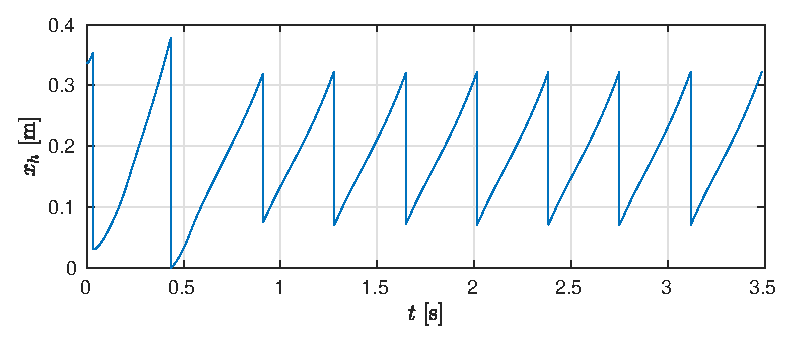
\includegraphics[width=\textwidth]{a04_x_h}
			\caption{horizontal position of the hip}
		\end{center}
	\end{subfigure}
	\begin{subfigure}[h]{0.6\textwidth}
		\begin{center}
			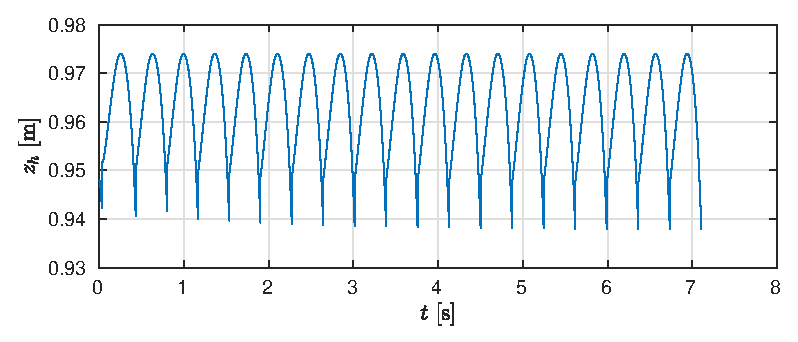
\includegraphics[width=\textwidth]{a04_z_h}
			\caption{vertical position of the hip}
		\end{center}
	\end{subfigure}
	\caption{Position of the hip as a function of time.}
	\label{fig::virtual_constraints_hip_position}
\end{figure}

The horizontal position increases steadily, while the vertical position bounces periodically.
This is good, since it indicates that the robot advances forward.
Let's note that on the horizontal position of the hip, the referential frame change is corrected.

\vspace{\baselineskip}

Then, let's look at the horizontal velocity of the hip, both the entire signal, and the velocity average over each step, on Figure~\ref{fig::virtual_constraints_hip_velocity}:

\begin{figure}[H]
	\begin{subfigure}[h]{0.35\textwidth}
		\begin{center}
			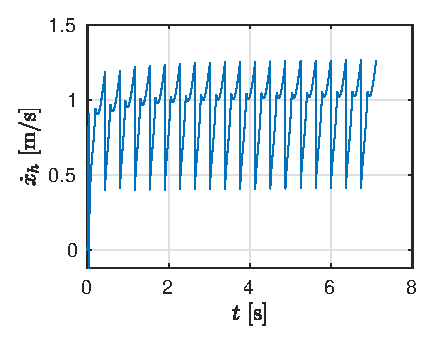
\includegraphics[width=\textwidth]{a04_dx_h}
			\caption{velocity of the hip}
		\end{center}
	\end{subfigure}
	\begin{subfigure}[h]{0.35\textwidth}
		\begin{center}
			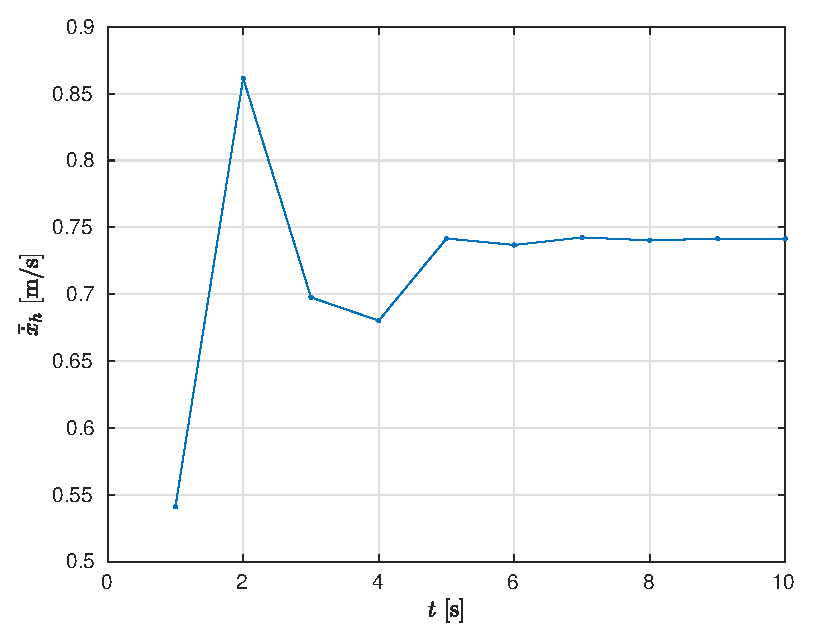
\includegraphics[width=\textwidth]{a04_average_dx_h}
			\caption{velocity of the hip averaged over the steps}
		\end{center}
	\end{subfigure}
	\caption{Velocity  of the hip in function of time / steps.}
	\label{fig::virtual_constraints_hip_velocity}
\end{figure}

The horizontal velocity of the hip stabilizes after the second step, and in the steady-state, oscillates between \SI{0.399}{\meter\per\second} and \SI{1.25}{\meter\per\second}, as can be seen on the left sub-figure.
When looking at the velocity averaged on each step (right sub-figure), we see that the average velocity in steady-state is $\sim\SI{0.88}{\meter\per\second}$ for a target of \SI{0.7}{\meter\per\second}.

\vspace{\baselineskip}

The plots of the step frequencies and durations (Figure~\ref{fig::virtual_constraints_step_regularity}) seem to indicate once again that the steady-state is reached after the second step.
The plots appear to vary until the fifth step, but the variations are negligible: in terms of step duration, after the second step, the variation doesn't exceed 2.7\%.

\begin{figure}[H]
	\begin{subfigure}[h]{0.35\textwidth}
		\begin{center}
			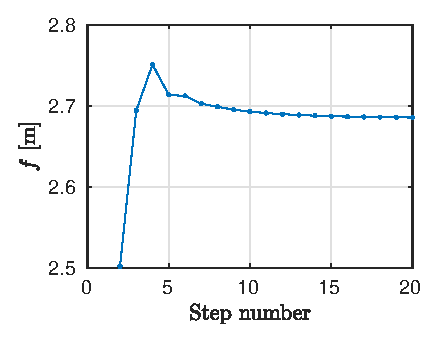
\includegraphics[width=\textwidth]{a04_step_frequency}
			\caption{step frequency}
		\end{center}
	\end{subfigure}
	\begin{subfigure}[h]{0.35\textwidth}
		\begin{center}
			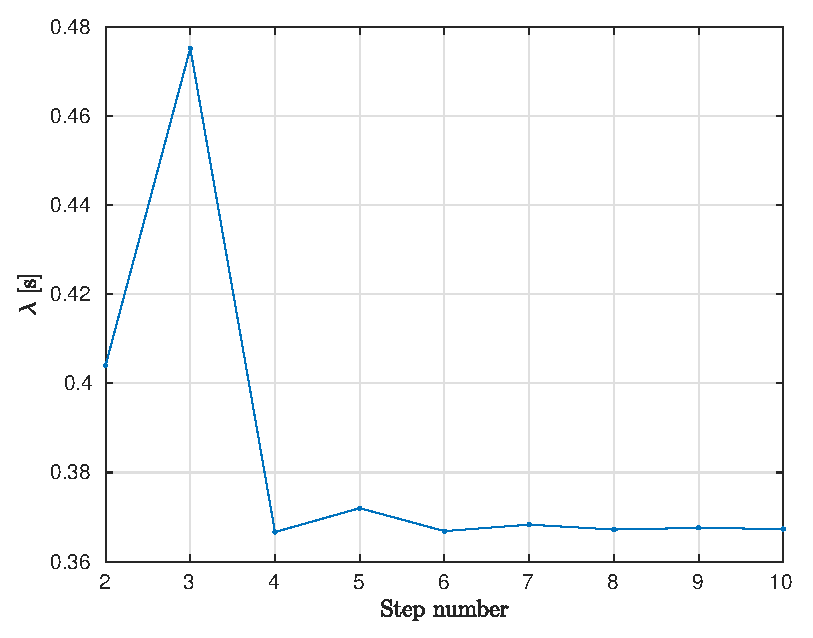
\includegraphics[width=\textwidth]{a04_step_lambda}
			\caption{step duration}
		\end{center}
	\end{subfigure}
	\caption{Regularity of the stepping.}
	\label{fig::virtual_constraints_step_regularity}
\end{figure}

The state-space plot displayed on Figure~\ref{img::virtual_constraints_state_space} indicates that the gait is stable after the second step.
Indeed, from step three and onwards, the state-space plots loop back on themselves.

\begin{figure}[H]
	\begin{subfigure}[h]{0.35\textwidth}
		\begin{center}
			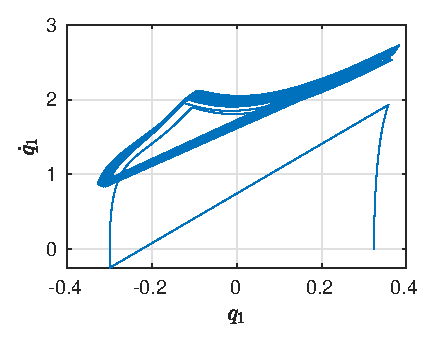
\includegraphics[width=\textwidth]{a04_state_space_q1_optimized}
			\caption{$q_1$ state-space plot}
		\end{center}
	\end{subfigure}
	\begin{subfigure}[h]{0.35\textwidth}
		\begin{center}
			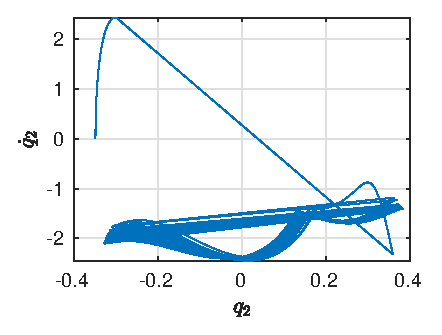
\includegraphics[width=\textwidth]{a04_state_space_q2_optimized}
			\caption{$q_2$ state-space plot}
		\end{center}
	\end{subfigure}

	\begin{subfigure}[h]{0.35\textwidth}
		\begin{center}
			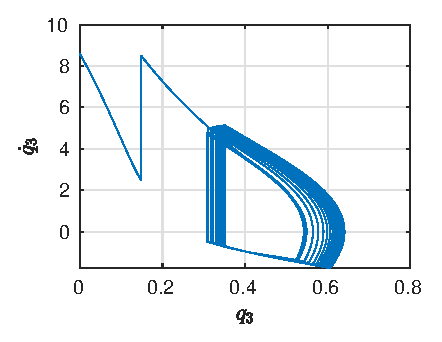
\includegraphics[width=\textwidth]{a04_state_space_q3_optimized}
			\caption{$q_3$ state-space plot}
		\end{center}
	\end{subfigure}
	\caption{State-space plot for the three generalized coordinates.}
	\label{img::virtual_constraints_state_space}
\end{figure}

Then, when looking at the command signals on Figure~\ref{fig::virtual_constraints_commands}, we see that the saturation affects $u_1$, but not $u_2$, because the latter doesn't reach \SI{30}{\newton\meter}:

\begin{figure}[H]
	\begin{subfigure}[h]{0.35\textwidth}
		\begin{center}
			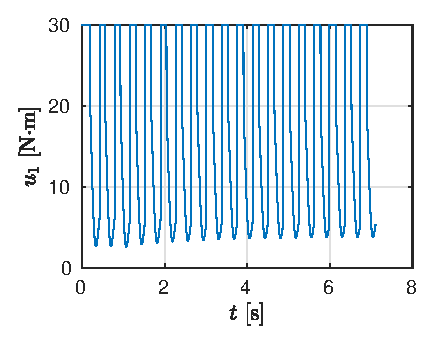
\includegraphics[width=\textwidth]{a04_control_torques_u1_optimized}
			\caption{first actuator}
		\end{center}
	\end{subfigure}
	\begin{subfigure}[h]{0.35\textwidth}
		\begin{center}
			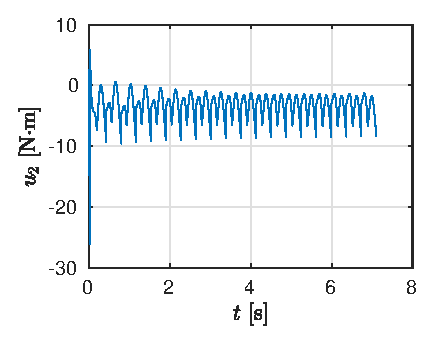
\includegraphics[width=\textwidth]{a04_control_torques_u2_optimized}
			\caption{second actuator}
		\end{center}
	\end{subfigure}
	\caption{Command angles in function of time for both actuators.}
	\label{fig::virtual_constraints_commands}
\end{figure}

Finally, the Table~\ref{tab::virtual_constraints_metrics} summarizes the numerical metrics about the gait:

\begin{table}[H]
	\sffamily
	\arrayrulecolor{white}
	\arrayrulewidth=1pt
	\renewcommand{\arraystretch}{1.5}
	\rowcolors[\hline]{1}{.!50!White}{}
	\centering
	\begin{tabular}{@{} A|B @{}}
		\cellcolor{ForestGreen}\arraycolor{White}\bfseries Metric  &
		\cellcolor{ForestGreen}\arraycolor{White}\bfseries Value \\
		\arraycolor{Black}
		step number					& 20 									\\
		normalized effort			& \SI{7.01}{\newton\meter\per\second}	\\
		CMT							& 2.29									\\
		$\dot{x}_\text{hip min}$	& \SI{0.399}{\meter\per\second}			\\
		$\dot{x}_\text{hip max}$	& \SI{1.25}{\meter\per\second}
	\end{tabular}
	\caption{Virtual constraints controller's numerical metrics.}
	\label{tab::virtual_constraints_metrics}
\end{table}

\newpage

\subsection{Virtual model controller}

The virtual model controller produces a very unexpected gait, from a qualitative point of view, quite the opposite from the virtual constraints controller.
One thing is that the swing leg passes over the torso, instead of in front of the stance leg in order to advance.
Another thing is that the transient-state is temporally short, but last approximately thirty steps, because initially, the bipedal robot is "tap dancing" of sorts.
Afterwards, the steady-state is smooth, although a little strange, with the swing leg swing over the top segment.

\vspace{\baselineskip}

The objective function~\ref{eq::virtual_model_objective_fun} was optimized with the following weights:

\begin{table}[H]
	\sffamily
	\arrayrulecolor{white}
	\arrayrulewidth=1pt
	\renewcommand{\arraystretch}{1.5}
	\rowcolors[\hline]{1}{.!50!White}{}
	\centering
	\begin{tabular}{@{} A|B @{}}
		\cellcolor{ForestGreen}\arraycolor{White}\bfseries Weight  &
		\cellcolor{ForestGreen}\arraycolor{White}\bfseries Value \\
		\arraycolor{Black}
		$w_1$					& 0								\\
		$w_2$					& 100							\\
		$w_3$					& 100							\\
		$w_4$					& 0								\\
		$w_5$					& 0								\\
		$w_6$					& 100							\\
		$\dot{x}_\text{hip d}$	& \SI{0.5}{\meter\per\second}	\\
		desired step length		& \SI{0.8}{\meter}
	\end{tabular}
	\caption{Virtual model controller's objective function's weights.}
\end{table}

so that the objective function becomes:

\begin{align*}
	\label{eq::virtual_model_objective_fun_final}
	f(p) &= w_2 | \dot{x}_\text{hip d} - \bar{\dot{x}}_\text{hip}(p) | + w_3 \text{CMT}(p)^2 + w_6 | \text{step length}_\text{d} - \text{step length}|
\end{align*}

and the following set of optimized parameters were obtained:

\begin{table}[H]
	\sffamily
	\arrayrulecolor{white}
	\arrayrulewidth=1pt
	\renewcommand{\arraystretch}{1.5}
	\rowcolors[\hline]{1}{.!50!White}{}
	\centering
	\begin{tabular}{@{} A|B @{}}
		\cellcolor{ForestGreen}\arraycolor{White}\bfseries Parameter  &
		\cellcolor{ForestGreen}\arraycolor{White}\bfseries Value \\
		\arraycolor{Black}
		$\dot{x}_\text{hip t}$	& \SI{1.563e-2}{\meter\per\second}	\\
		$k_{d x_\text{hip}}$	& \num{1.763e2}			\\
		$k_{p x_\text{top}}$	& 33.34					\\
		$k_{d x_\text{top}}$	& \num{1.121e2}			\\
		$\alpha$				& \SI{0.5062}{\radian}	\\
		$k_{p x_\text{swf}}$	& 2						\\
		$k_{d x_\text{swf}}$	& 0.06250				\\
		$k_{p z_\text{swf}}$	& 52.43					\\
		$k_{d z_\text{swf}}$	& 0.5178				\\
		step length				& \SI{0.5519}{\meter}
	\end{tabular}
	\caption{Virtual model controller's optimized parameters.}
\end{table}

\newpage

First, let's look at the position of the hip along the time on Figure~\ref{fig::virtual_model_hip_position}:

\begin{figure}[H]
	\begin{subfigure}[h]{0.6\textwidth}
		\begin{center}
			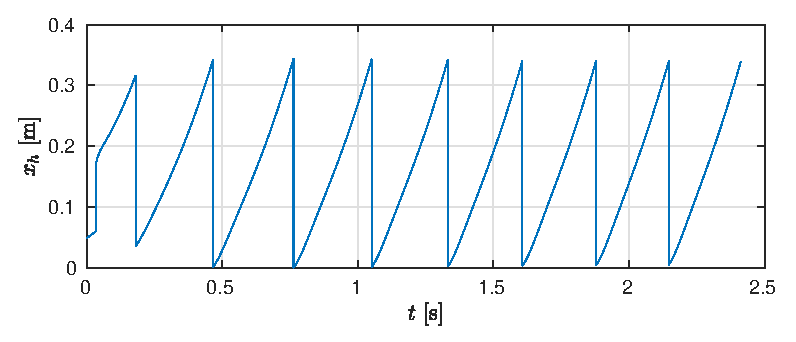
\includegraphics[width=\textwidth]{a05_x_h}
			\caption{horizontal position of the hip}
		\end{center}
	\end{subfigure}
	\begin{subfigure}[h]{0.6\textwidth}
		\begin{center}
			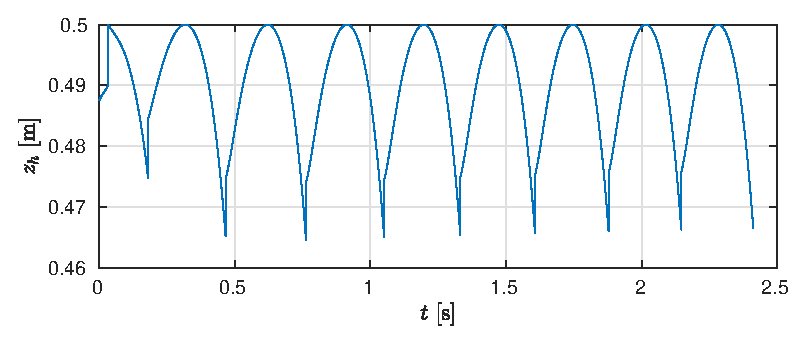
\includegraphics[width=\textwidth]{a05_z_h}
			\caption{vertical position of the hip}
		\end{center}
	\end{subfigure}
	\caption{Position of the hip as a function of time.}
	\label{fig::virtual_model_hip_position}
\end{figure}

The horizontal position increases steadily, while the vertical position bounces periodically.
This is good, since it indicates that the robot advances forward. Let's note that on the horizontal position of the hip, the referential frame change is corrected.

\vspace{\baselineskip}

Then, let's look at the horizontal velocity of the hip, both the entire signal, and the velocity average over each step, on Figure~\ref{fig::virtual_model_hip_velocity}:

\begin{figure}[H]
	\begin{subfigure}[h]{0.35\textwidth}
		\begin{center}
			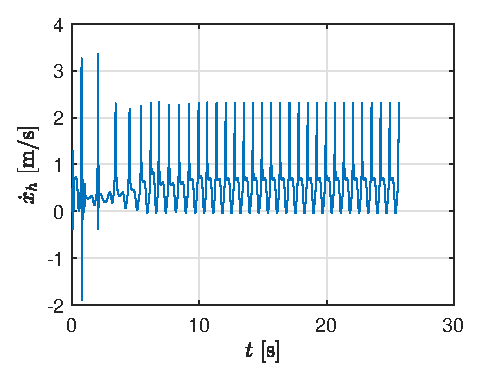
\includegraphics[width=\textwidth]{a05_dx_h}
			\caption{velocity of the hip}
		\end{center}
	\end{subfigure}
	\begin{subfigure}[h]{0.35\textwidth}
		\begin{center}
			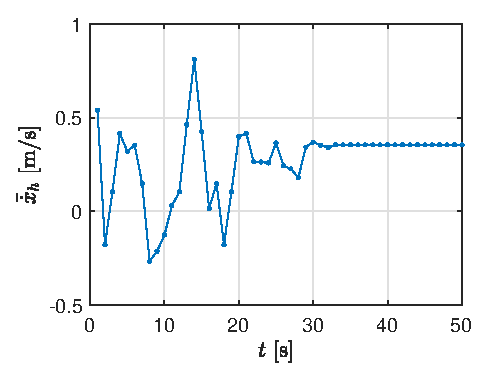
\includegraphics[width=\textwidth]{a05_average_dx_h}
			\caption{velocity of the hip averaged over the steps}
		\end{center}
	\end{subfigure}
	\caption{Velocity  of the hip in function of time / steps.}
	\label{fig::virtual_model_hip_velocity}
\end{figure}

We can see on the right sub-figure that the horizontal velocity of the hip stabilizes after the thirtieth step.
In the steady-state, it oscillates between \SI{-0.0541}{\meter\per\second} and \SI{2.23}{\meter\per\second}, as can be seen on the left sub-figure.
When looking at the velocity averaged on each step (right sub-figure), we see that the average velocity in steady-state is $\sim\SI{0.40}{\meter\per\second}$ for a target of \SI{0.5}{\meter\per\second}.

\vspace{\baselineskip}

The plots of the step frequencies and durations (Figure~\ref{fig::virtual_constraints_step_regularity}) seem to indicate once again that the steady-state is reached after the thirtieth step.

\begin{figure}[H]
	\begin{subfigure}[h]{0.35\textwidth}
		\begin{center}
			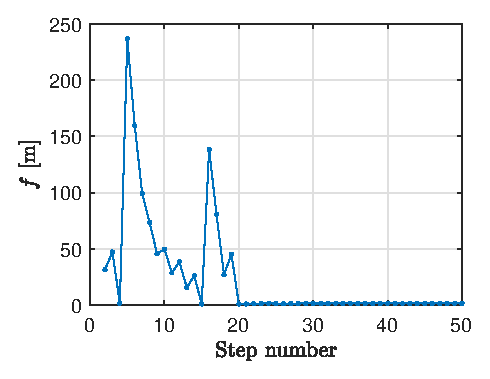
\includegraphics[width=\textwidth]{a05_step_frequency}
			\caption{step frequency}
		\end{center}
	\end{subfigure}
	\begin{subfigure}[h]{0.35\textwidth}
		\begin{center}
			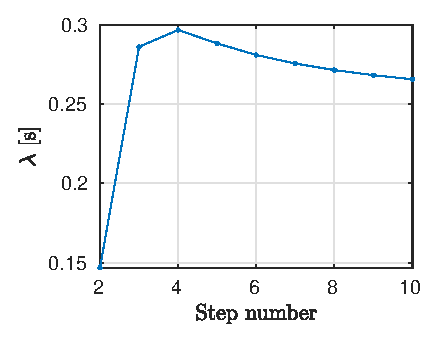
\includegraphics[width=\textwidth]{a05_step_lambda}
			\caption{step duration}
		\end{center}
	\end{subfigure}
	\caption{Regularity of the stepping.}
	\label{fig::virtual_model_step_regularity}
\end{figure}

The state-space plot displayed on Figure~\ref{img::virtual_model_state_space} indicates that the gait is stable after the many steps, but the exact number cannot be confirmed on those plots alone, although the previous Figures indicate that if we could count, it would probably be 30.

\begin{figure}[H]
	\begin{subfigure}[h]{0.35\textwidth}
		\begin{center}
			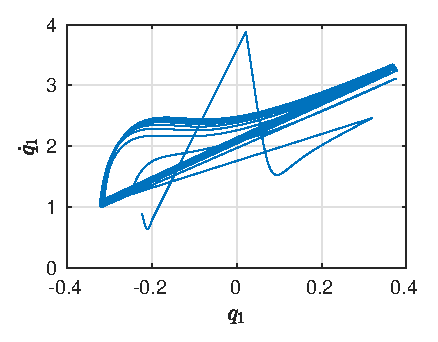
\includegraphics[width=\textwidth]{a05_state_space_q1_optimized}
			\caption{$q_1$ state-space plot}
		\end{center}
	\end{subfigure}
	\begin{subfigure}[h]{0.35\textwidth}
		\begin{center}
			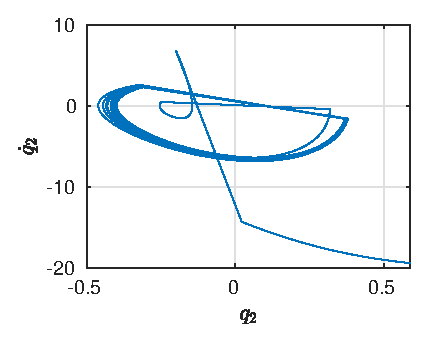
\includegraphics[width=\textwidth]{a05_state_space_q2_optimized}
			\caption{$q_2$ state-space plot}
		\end{center}
	\end{subfigure}

	\begin{subfigure}[h]{0.35\textwidth}
		\begin{center}
			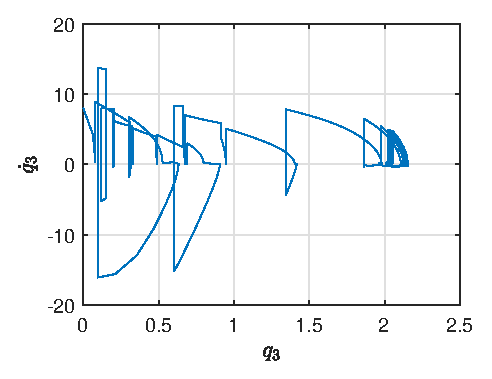
\includegraphics[width=\textwidth]{a05_state_space_q3_optimized}
			\caption{$q_3$ state-space plot}
		\end{center}
	\end{subfigure}
	\caption{State-space plot for the three generalized coordinates.}
	\label{img::virtual_model_state_space}
\end{figure}

Then, when looking at the command signals on Figure~\ref{fig::virtual_model_commands}, we see that the saturation affects both commands:

\begin{figure}[H]
	\begin{subfigure}[h]{0.35\textwidth}
		\begin{center}
			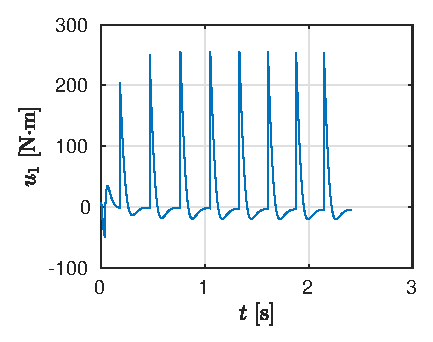
\includegraphics[width=\textwidth]{a05_control_torques_u1_optimized}
			\caption{first actuator}
		\end{center}
	\end{subfigure}
	\begin{subfigure}[h]{0.35\textwidth}
		\begin{center}
			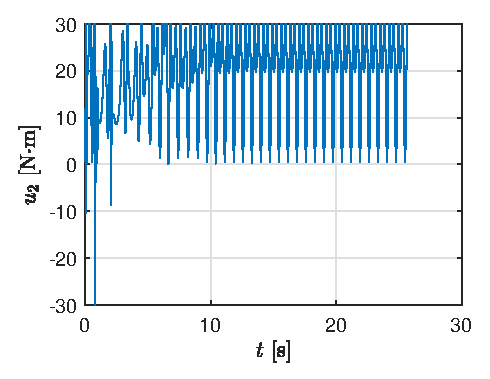
\includegraphics[width=\textwidth]{a05_control_torques_u2_optimized}
			\caption{second actuator}
		\end{center}
	\end{subfigure}
	\caption{Command angles in function of time for both actuators.}
	\label{fig::virtual_model_commands}
\end{figure}

Finally, the Table~\ref{tab::virtual_model_metrics} summarizes the numerical metrics about the gait:

\begin{table}[H]
	\sffamily
	\arrayrulecolor{white}
	\arrayrulewidth=1pt
	\renewcommand{\arraystretch}{1.5}
	\rowcolors[\hline]{1}{.!50!White}{}
	\centering
	\begin{tabular}{@{} A|B @{}}
		\cellcolor{ForestGreen}\arraycolor{White}\bfseries Metric  &
		\cellcolor{ForestGreen}\arraycolor{White}\bfseries Value \\
		\arraycolor{Black}
		step number					& 50									\\
		normalized effort			& \SI{12.3}{\newton\meter\per\second}	\\
		CMT							& 0.917									\\
		$\dot{x}_\text{hip min}$	& \SI{-0.0467}{\meter\per\second}		\\
		$\dot{x}_\text{hip max}$	& \SI{2.32}{\meter\per\second}
	\end{tabular}
	\caption{Virtual model controller's numerical metrics.}
	\label{tab::virtual_model_metrics}
\end{table}

When applying external forces to the robot, as described in the methods (a force applied for \SI{0.2}{\second} at the beginning of a steady-state step), we observe that the robot falls back to "tap dancing" transiently, before reaching a steady-state again.
This can mostly be seen on the step length plot on Figure~\ref{fig::virtual_model_external_forces}, where the "tap dancing" and the walking by swinging the foot over the top link can be very easily distinguished:

\begin{figure}[H]
	\begin{subfigure}[h]{0.35\textwidth}
		\begin{center}
			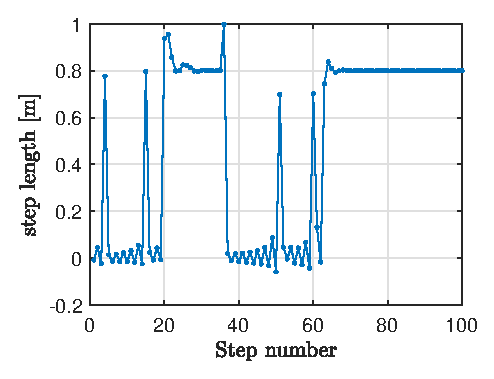
\includegraphics[width=\textwidth]{a05_step_length_F100}
			\caption{\SI{100}{\newton} pushing}
		\end{center}
	\end{subfigure}
	\begin{subfigure}[h]{0.35\textwidth}
		\begin{center}
			\includegraphics[width=\textwidth]{a05_step_length_F_15}
			\caption{\SI{15}{\newton} pull}
		\end{center}
	\end{subfigure}

	\begin{subfigure}[h]{0.35\textwidth}
		\begin{center}
			\includegraphics[width=\textwidth]{a05_step_length}
			\caption{without an external force}
		\end{center}
	\end{subfigure}
	\caption{Step length with and without an external force applied at the hip.}
	\label{fig::virtual_model_external_forces}
\end{figure}

The values for the forces were chosen so that the robot would have time to go back to a steady-state before reaching step 100.

\vspace{\baselineskip}

The variance values for the measuring noise were chosen at the limit before the numerical integration to solve the equation of movement stop working properly.
This means that unfortunately, there are not plots or measures for when it stops to work, while when it works, the plots are essentially indistinguishable from when there is no noise.
To recall, the gaussian noise is centered, so the mean is null.
The variance is of 0.01 for $q_i$ and 0.1 for $\dot{q}_i$.
It was applied sequentially, one angle or angle rate at a time.

